\documentclass[final,3p,times,twocolumn]{elsarticle}

\usepackage{amsmath,amssymb,amsthm}
\usepackage{url}
\usepackage{graphicx}
\usepackage{booktabs}
\usepackage{enumitem}
\usepackage{xcolor}
\newcommand{\rev}[1]{\textcolor{blue}{#1}}  % all changes; redefine as #1 to hide
\newcommand{\revb}[1]{\textcolor{blue}{#1}} % all changes; redefine as #1 to hide
\newcommand{\revc}[1]{\textcolor{blue}{#1}} % all changes; redefine as #1 to hide
\newcommand{\revd}[1]{\textcolor{blue}{#1}} % all changes; redefine as #1 to hide
\setlist[itemize]{itemsep=1pt, topsep=2pt, parsep=0pt, partopsep=0pt}

\newtheorem{proposition}{Proposition}
\newtheorem{assumption}{Assumption}
\newtheorem{remark}{Remark}
\newtheorem{definition}{Definition}

\journal{Journal of Process Control}

\begin{document}

\begin{frontmatter}

\title{Model-Free PID Tuning via Encirclements of the Step Response}

\author[inst1]{Daniel Pachner}
\author[inst1]{Pavel Otta\corref{cor1}}
\ead{pavel.otta@cvut.cz}
\author[inst1]{Ji\v{r}\'{\i} Dost\'al}
\author[inst2]{\rev{Vladim\'{\i}r Havlena}}

\cortext[cor1]{Corresponding author}

\affiliation[inst1]{organization={University Centre for
Energy Efficient Buildings (UCEEB), Czech Technical University in
Prague}, city={Bu\v{s}t\v{e}hrad}, country={Czech Republic}}
\affiliation[inst2]{organization={Department of Control Engineering,
Faculty of Electrical Engineering, Czech Technical University in Prague},
city={Prague}, country={Czech Republic}}

\begin{abstract}
\revc{From one closed-loop step response, three phase portraits of the
control error are formed---error against its running integral, first
difference, and second difference---and the winding number of each
about its settling point is counted. The counts are invariant to time
and amplitude scaling, so fixed dimensionless thresholds serve every
loop, and they are band-selective: they locate insufficient damping in
the low-, mid-, and high-frequency bands owned by the integral,
proportional, and derivative channels. A settling-anchored window makes
the counts independent of the observation length; a parameter-free
stability screen halves all gains when the record fails to settle, so
the method bootstraps from arbitrary initial gains. A triangular rule
cuts the lowest violated band---the only one whose blame is
unambiguous---raises the verified-clean bands below it, and with all
portraits clean raises all bands. The iteration is deterministic,
bounded by construction, and exploration-free\revd{---safe on a
process in operation---}and it converges to a
limit cycle on the boundary of the well-damped tuning set; the required
monotonicity is derived from the plant class near the boundary. The
method rests on two assumptions---a stable, self-regulating process of
the first-order-plus-time-delay class and a controller from the nested
family $\mathrm{I} \subset \mathrm{PI} \subset \mathrm{PID}$ with
mandatory integral action---and is validated on a battery of
process-typical plants with identical defaults throughout\revd{;
each iteration costs one routine setpoint step, and every decision is
visible in the three portraits}. A reference
implementation is public.}
\end{abstract}

\begin{highlights}
\item A deterministic reading of the step response replaces manual PID
tuning.
\item Three phase portraits of the control error give a dimensionless
damping diagnostic.
\item The diagnostic is band-selective, assigning oscillation to the I,
P, or D channel.
\item A well-posedness guard keeps the encirclement count independent
of window length.
\item One triangular rule converges to the boundary of the well-damped
tuning set.
\end{highlights}

\begin{keyword}
PID control \sep controller tuning \sep data-driven control \sep
phase plane \sep step response
\end{keyword}

\end{frontmatter}

%=====================================================================
\section{Introduction}
%=====================================================================

Eighty years after Ziegler and Nichols \cite{ZN1942}, PID remains the
dominant industrial controller \cite{AstromHagglund2001}, and most PID
loops are still tuned by inspection: an engineer steps the setpoint,
looks at the response, and adjusts a gain by feel. The literature's two
remedies both discard the inspection. Model-based rules---Ziegler--Nichols
\cite{ZN1942}, Cohen--Coon \cite{CohenCoon1953}, IMC \cite{RiveraIMC},
SIMC \cite{Skogestad2003}---replace it with an identified low-order model
and inherit that model's errors. \rev{Both experimental legs of
Ziegler--Nichols have since been revisited with modern robustness tools:
\r{A}str\"om and H\"agglund \cite{AstromHagglund2004} rederived the
step-response method from the standpoint of robust loop shaping,
obtaining simple tuning rules with guaranteed robustness for essentially
monotone processes, while Schlegel and co-workers
\cite{SchlegelCech2005,Schlegel2011} revisited the frequency-response
method, developing robust PID design over sets of plants that share a
structural constraint---for example, a single common point of the
frequency response.} Data-driven schemes replace it with a
criterion and the machinery to serve it: a dedicated relay experiment
that deliberately excites a sustained oscillation
\cite{AstromHagglund1984}, gradient experiments on a quadratic cost
\cite{HjalmarssonIFT}, a one-shot identification-like problem
\cite{CampiVRFT}, or online perturbation of the gains
\cite{KillingsworthKrstic}. The inspection itself---which gain is to
blame, given this response---has remained tacit.

This paper formalizes the inspection. The contributions are:
(i)~a triple of phase portraits of the control error whose encirclement
counts form a dimensionless, scale-free, band-selective damping diagnostic
(Section~\ref{sec:feature});
(ii)~a well-posedness analysis of the counts, including a counterexample
showing that a na\"ively windowed count diverges, and a settling-anchored
guard that provably restores window independence
(Section~\ref{sec:wellposed});
(iii)~a single triangular tuning rule in band-ordered gain coordinates,
interpreted as band-wise
loop shaping, with boundedness unconditional and boundary convergence
\revb{under a monotonicity property derived from the plant class
(Proposition~\ref{prop:mono}, Section~\ref{sec:rule})};
(iv)~validation on a battery of process-typical plants with identical
default parameters throughout (Section~\ref{sec:battery}).

The method claims no optimality: it returns a fast, well-damped
tuning---the contract an expert tuner offers---in exchange for one
closed-loop setpoint step per iteration and nothing else. No model, no
relay experiment, no solver; and full auditability, since an operator
watching the three plots sees exactly what the algorithm sees.
\revd{The whole method carries five dimensionless constants
(Table~\ref{tab:defaults}), none adjusted for any plant.}

\revc{Every move either repairs a diagnosed fault or tightens all
gains by one verified notch---no iterate is an exploration step---so
the tuner runs safely on a process in operation. Adaptive and
learning-based tuners must operate the plant under unvetted or
perturbed controllers to acquire information
\cite{HjalmarssonIFT,KillingsworthKrstic}; here information is a
by-product of a routine setpoint step under the current controller.
Figures~\ref{fig:init_step}--\ref{fig:tuned_portraits} show the method
on one plant (P2, Section~\ref{sec:battery}), from a severely
mis-tuned start, before any mathematics: response and portraits before
tuning and after, captured from the running implementation (Data
availability).}

\begin{figure*}[t]
\centering
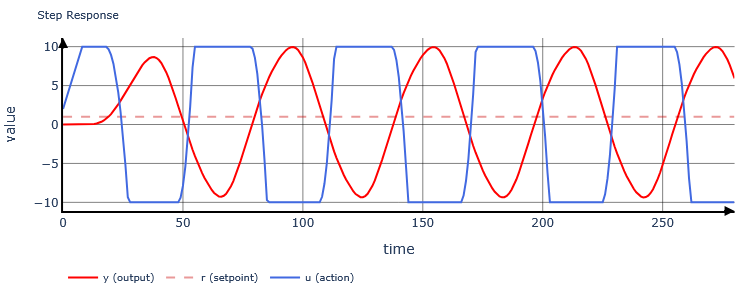
\includegraphics[width=0.85\textwidth]{init_step.png}
\caption{Step response before tuning. The mis-tuned derivative channel
sustains an oscillation with the actuator railing between its limits;
nothing here suggests which gain is at fault.}
\label{fig:init_step}
\end{figure*}

\begin{figure*}[t]
\centering
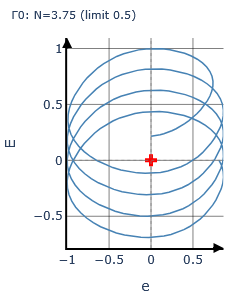
\includegraphics[width=0.32\textwidth]{init_F0.png}\hfill
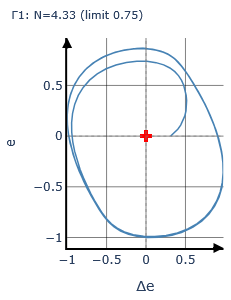
\includegraphics[width=0.32\textwidth]{init_F1.png}\hfill
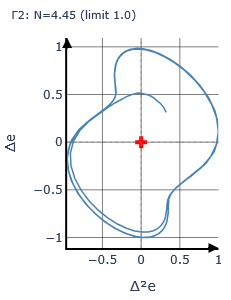
\includegraphics[width=0.32\textwidth]{init_F2.png}
\caption{Portraits before tuning, left to right $\Gamma_0,\Gamma_1,\Gamma_2$.
All three loop well past their limits
($N_0{=}3.75$ vs.\ $0.5$; $N_1{=}4.33$ vs.\ $0.75$; $N_2{=}4.45$ vs.\
$1.0$)---the response of Figure~\ref{fig:init_step} is unreadable, but
here the fault is explicit in every band at once.}
\label{fig:init_portraits}
\end{figure*}

\begin{figure*}[t]
\centering
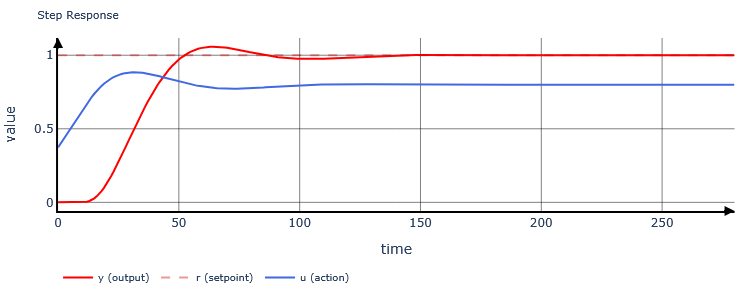
\includegraphics[width=0.85\textwidth]{tuned_step.png}
\caption{Step response after tuning: a single overshoot settling
cleanly to the setpoint, actuator unsaturated.}
\label{fig:tuned_step}
\end{figure*}

\begin{figure*}[t]
\centering
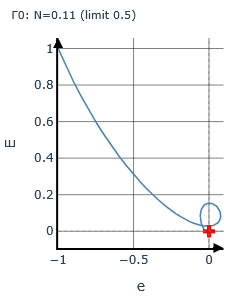
\includegraphics[width=0.32\textwidth]{tuned_F0.png}\hfill
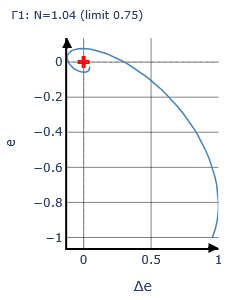
\includegraphics[width=0.32\textwidth]{tuned_F1.png}\hfill
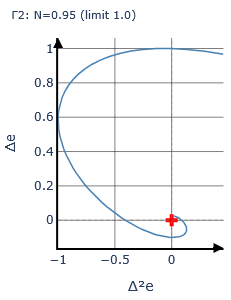
\includegraphics[width=0.32\textwidth]{tuned_F2.png}
\caption{Portraits after tuning. $\Gamma_2$ is now within its limit
($0.95$ vs.\ $1.0$); $\Gamma_0,\Gamma_1$ have fallen sharply from
Figure~\ref{fig:init_portraits} ($3.75\to1.11$, $4.33\to0.99$) and sit
just outside theirs, the boundary limit cycle of
Proposition~\ref{prop:conv} caught mid-oscillation rather than a rare
failure to converge.}
\label{fig:tuned_portraits}
\end{figure*}

%=====================================================================
\section{The encirclement features}
\label{sec:feature}
%=====================================================================

The method rests on exactly two standing assumptions, stated once and
used throughout.

\begin{assumption}[Process class]\label{ass:plant}
The process is a stable, self-regulating SISO plant whose open-loop step
response is essentially monotone with dead time---the class adequately
captured by first-order-plus-time-delay (FOPTD) models. FOPTD is meant
here as a modelling class, not a literal transfer-function restriction:
higher-order overdamped dynamics belong to it.
\end{assumption}

\revc{``Essentially monotone'' admits mild non-monotonicity; the
construction extends to plants with damped open-loop oscillations
provided a well-damped tuning exists within the gain box and the
monotonicity of Proposition~\ref{prop:mono} holds there. What excludes
a plant is a resonance strong enough that reducing a band's gain fails
to damp that band. The propositions below are proved on the strictly
monotone core of the class; a checkable characterization of the wider
admissible set, in the spirit of
\cite{SchlegelCech2005,Schlegel2011}, is left open.}

\revc{The proofs below use the frequency-domain content of the
FOPTD core of Assumption~\ref{ass:plant}: both $|G(j\omega)|$ and
$\arg G(j\omega)$ strictly decrease on $(0,\infty)$, with
$\arg G \to -\infty$ (dead time); for the canonical member
$|G| = K/\sqrt{1+\omega^2T^2}$,
$\arg G = -\arctan\omega T - \omega L$. Monotone \emph{phase} makes
the loss of closed-loop damping a single-frequency event
(Proposition~\ref{prop:pair}); monotone \emph{gain} orders the bands
the controller channels own (Proposition~\ref{prop:band}). One
structural fact joins them: $C$ is linear in its gains, so scaling all
three by $m$ maps $L = CG$ to $mL$---the Nyquist locus changes
magnitude, not shape.}

\begin{assumption}[Controller structure]\label{ass:pid}
The controller is drawn from the nested family
$\mathrm{I} \subset \mathrm{PI} \subset \mathrm{PID}$: a parallel
structure $u = K_p e + K_i\!\int\! e + K_d \dot e$ in a unity-feedback
loop, with the integral channel mandatory ($K_i > 0$) and the
proportional and derivative channels optional ($K_p, K_d \ge 0$).
\end{assumption}

\rev{Nothing else is assumed: no model, no noise model, no excitation
beyond routine setpoint steps under the existing controller. The
mandatory integral channel is what drives $e \to 0$ at steady state and
thus lets the portraits below terminate at the origin; its necessity is
made precise after Definition~\ref{def:count}.}

A tuning experiment applies a setpoint step and
records the error $e_k$, $k = 0,\dots,K$, at period $T_s$, over a window
in which the response settles. Form the running integral $E_k$ and the
differences $\Delta e_k$, $\Delta^2 e_k$, and pair each signal with its
own difference:
\begin{align}
\Gamma_0&: \bigl(e_k,\, E_k{-}E_{K}\bigr), \notag\\
\Gamma_1&: \bigl(\Delta e_k,\, e_k\bigr), \notag\\
\Gamma_2&: \bigl(\Delta^2 e_k,\, \Delta e_k\bigr).
\label{eq:plots}
\end{align}
$\Gamma_1$ is the classical phase plane of the error; $\Gamma_0$ and
$\Gamma_2$ are its integrated and differentiated siblings; all three
terminate at the origin when the loop settles. \revc{We call
\eqref{eq:plots} \emph{Pachner plots}, after the first author, who
devised the construction.}

A well-damped loop spirals into the origin without completing a turn; an
under-damped loop encircles it. The count is made precise as follows.

\begin{definition}[Encirclement count]\label{def:count}
Given a planar trajectory $(x_k, y_k)$, $k = 0,\dots,J$:
(i) normalize each coordinate by its peak magnitude, mapping the curve
into $[-1,1]^2$;
(ii) truncate at the last entry into the disc of radius
$\varepsilon \in (0,1)$ about the origin;
(iii) define $N$ as the winding number of the remaining curve about the
origin: total swept angle over $2\pi$, evaluated as the endpoint angle
difference corrected by signed crossings of the negative horizontal
semi-axis. Partial revolutions count fractionally.
\end{definition}

\rev{Definition~\ref{def:count} presupposes that the trajectory
terminates at the origin, which the integral channel guarantees:
$e \to 0$ for every stable tuning of Assumption~\ref{ass:pid}. Without
it, a P-only loop on a self-regulating plant settles at a nonzero
offset, $\Gamma_0$ and $\Gamma_1$ terminate away from the origin,
truncation never triggers, and the winding number measures the wrong
quantity. This is the concrete content of requiring $K_i > 0$.}

Applying Definition~\ref{def:count} to $\Gamma_0, \Gamma_1, \Gamma_2$
yields the feature vector $\mathbf N(\theta) = (N_0, N_1, N_2)$ at
controller setting $\theta = (K_p, K_i, K_d)$, from a single step test,
with no plant knowledge.

\begin{proposition}[Invariance]\label{prop:invariance}
$\mathbf N$ is invariant under time reparametrization $t \mapsto \alpha t$,
$\alpha > 0$, of the underlying response, and under independent positive
scaling of either coordinate of each trajectory---in particular under
scaling of the setpoint step and, in the fast-sampling limit, of the
sampling period.
\end{proposition}

\begin{proof}
The winding number depends only on the oriented image of the curve, not
its parametrization; per-axis peak normalization removes amplitude and
units, and the truncation disc is defined on normalized coordinates.
\end{proof}

\begin{sloppypar}
Consequently one threshold set serves all loops: the defaults
$\bar{\mathbf N} = (0.5, 0.75, 1.0)$ together with $\varepsilon = 0.1$
are used unchanged in every result of this paper. They function as the
definition of ``well damped,'' not as tuning knobs.
\end{sloppypar}

\revc{Which damping the counts read, and why a single one
dominates, is a consequence of the plant class.}

\begin{proposition}[Critical pair]\label{prop:pair}
\revd{Let $G$ satisfy Assumption~\ref{ass:plant} and scale all
gains together, $L \mapsto mL$, $m>0$. The loop is stable up to a
finite $m^\ast$ and loses stability there through one complex pole
pair, at the phase-crossover frequency $\omega_{180}$---the maximizer
of $|L(j\omega)|$ over $\{\omega:\arg L(j\omega)=-\pi\}$. Near
$m^\ast$ this pair is the least damped in the loop, and its damping
$\zeta(m)$ decreases continuously to zero as $m\uparrow m^\ast$.}
\end{proposition}

\begin{proof}
\revd{$\arg C \in [-\pi/2,\pi/2]$ while $\arg G \to -\infty$, so
$\arg L$ reaches $-\pi$ at frequencies bounded away from $0$ and
$\infty$. Growing $m$ scales the locus $mL$ radially; it first touches
$-1$ at $m^\ast = 1/|L(j\omega_{180})|$, generically at one frequency.
The touch is transversal ($\partial|mL|/\partial m = |L| > 0$), so one
conjugate pair crosses the imaginary axis at $\omega_{180}$ while all
other poles keep strictly positive damping nearby; continuity in $m$
gives the strict decrease of $\zeta(m)$.}
\end{proof}

\revd{So near the boundary one pair carries the ringing; write}
\begin{equation}
e(t) = A\,e^{-\alpha t}\cos(\omega t+\varphi) + r(t),
\qquad \zeta = \frac{\alpha}{\sqrt{\alpha^2+\omega^2}},
\label{eq:mode}
\end{equation}
\revd{with $r$ the remaining, faster-settling part of the error. The
decomposition is exact as $m \uparrow m^\ast$; between the well-damped
boundary and the stability boundary---where the rule operates---it is
the working model, validated in Section~\ref{sec:battery}. The
propositions below read \eqref{eq:mode}.}

\begin{proposition}[Damping law]\label{prop:law}
\revb{For the mode of \eqref{eq:mode}, each truncated portrait of
Definition~\ref{def:count} winds
\begin{equation}
N = \frac{\ln(1/\varepsilon)}{2\pi}\,
\frac{\sqrt{1-\zeta^2}}{\zeta} + \eta,
\qquad \revc{|\eta| < 1,}
\label{eq:law}
\end{equation}
where $\eta$ is a fractional endpoint term. The map $\zeta\mapsto N$
is strictly decreasing on $(0,1)$; each threshold crossing
$N_k=\bar N_k$ therefore occurs at a unique damping $\bar\zeta_k$.}
\end{proposition}

\begin{proof}
\revb{Differentiation multiplies the mode by the fixed complex number
$-\alpha+j\omega$, so each portrait is a fixed linear image of the
mode's phase plane; a linear isomorphism preserves oriented loops, and
all three portraits trace one logarithmic spiral up to linear
equivalence. From its peak to the last entry into the
$\varepsilon$-disc the spiral's radius contracts by $\varepsilon$,
taking time $\alpha^{-1}\ln(1/\varepsilon)$, i.e.\
$(\ln(1/\varepsilon)/2\pi)(\omega/\alpha)$ revolutions, and
$\omega/\alpha=\sqrt{1-\zeta^2}/\zeta$; the truncated endpoints
contribute less than a half-turn each. Monotonicity:
$\mathrm d(\sqrt{1-\zeta^2}/\zeta)/\mathrm d\zeta<0$ on
$(0,1)$.}
\end{proof}

\revd{Hence $N_k>\bar N_k \iff \zeta<\bar\zeta_k$: ``rings'' is a
sign test, scale- and clock-free by
Proposition~\ref{prop:invariance}. The rule uses only the sign;
inverting \eqref{eq:law} gives a free damping estimator. Sampling
shifts the constant in \eqref{eq:law}---most in $\Gamma_2$---but never
the monotonicity, so the damping specifications are
\emph{calibrated}, not derived: the measured $N_k(\zeta)$ of the exact
second-order step error crosses $\bar{\mathbf N}=(0.5,0.75,1.0)$ at
$\bar\zeta \approx 0.64,\,0.49,\,0.24$ ($\varepsilon=0.1$), strictest
in the lowest band. For a clean dominant mode the count is set by
$\varepsilon$; the settling window of Section~\ref{sec:wellposed} only
guards against noise-dominated tails.}

\begin{proposition}[Band selectivity and upward leakage]\label{prop:band}
\revd{Write $e = x + r$ as in \eqref{eq:mode}. Each differencing
step multiplies the mode by its natural frequency
$\omega_n=\sqrt{\alpha^2+\omega^2}$ and the essentially monotone
residual only by its slower decay rate $\alpha_r<\omega_n$; each
integration does the reverse. A mode's visibility in $\Gamma_j$ thus
grows by $\omega_n/\alpha_r>1$ per band index: it is most visible in
its own band, visible in every band above, and invisible below. The
set of bands whose count a mode lifts is upward-closed,
$\{k,k{+}1,\dots\}$, and several modes superpose, each
upward-closed.}
\end{proposition}

The bands are owned by the controller channels: for the parallel PID,
$|C(j\omega)| \approx K_i/\omega$ at low frequency, $\approx K_p$ in the
mid band, $\approx K_d\omega$ at high frequency. Hence $N_0$ indicts
$K_i$, $N_1$ indicts $K_p$, $N_2$ indicts $K_d$. This correspondence is
the entire basis of the tuning rule.

\emph{Attribution.} \revb{The violated set is a union of
upward-closed sets (Proposition~\ref{prop:band}), so its lowest member
is the unique band whose violation cannot be leakage---nothing exists
below it to leak in---while violations above it are evidentially void:
a genuine upper-band mode and upward leakage produce indistinguishable
counts. Synthetically, one under-damped mid mode alone gives
$\mathbf N = (0.12,\, 3.9,\, 6.5)$---the high count exceeds the mid
one purely by leakage---while a lone high mode gives
$(0.12,\, 0.05,\, 5.7)$, leaking nowhere below. The rule of
Section~\ref{sec:rule} is built on this asymmetry.}

%=====================================================================
\section{Well-posedness of the count}
\label{sec:wellposed}
%=====================================================================

\rev{Per-axis normalization buys Proposition~\ref{prop:invariance} but
blinds each portrait to absolute scale. A persistent
micro-oscillation---quantization, a marginally damped parasitic mode,
numerical residue at a fraction of a percent of the step---can dominate
$\Delta e$, $\Delta^2 e$ long after $e$ has settled; normalized to its
own peak, the ripple fills the portrait and winds indefinitely, so the
count grows with the observation window and threshold comparisons become
artefacts of the window.}

This is not hypothetical. For the plant $P(s) = e^{-4s}/(8s+1)^6$ at
gains reached mid-iteration by the tuning rule, the response settles to
$|e| < 0.005$ (peak $1.0$) well inside the default window, yet the counts
evaluate to $\mathbf N = (0.12,\, 1.84,\, 2.86)$ on that window,
$(0.62,\, 9.22,\, 17.2)$ on a window six times longer, and
$(0.62,\, 17.3,\, 37.3)$ on twice that: $N_1, N_2$ grow essentially
linearly in window length. In closed loop the consequence is erratic:
threshold comparisons flip under $10\%$ gain changes and the corrective
moves of the tuning rule fight each other without
converging. Figure~\ref{fig:wellposed} shows the pattern: unguarded
counts climb without bound as the window lengthens, while the guarded
counts defined next sit flat.

\begin{figure}[h]
\centering
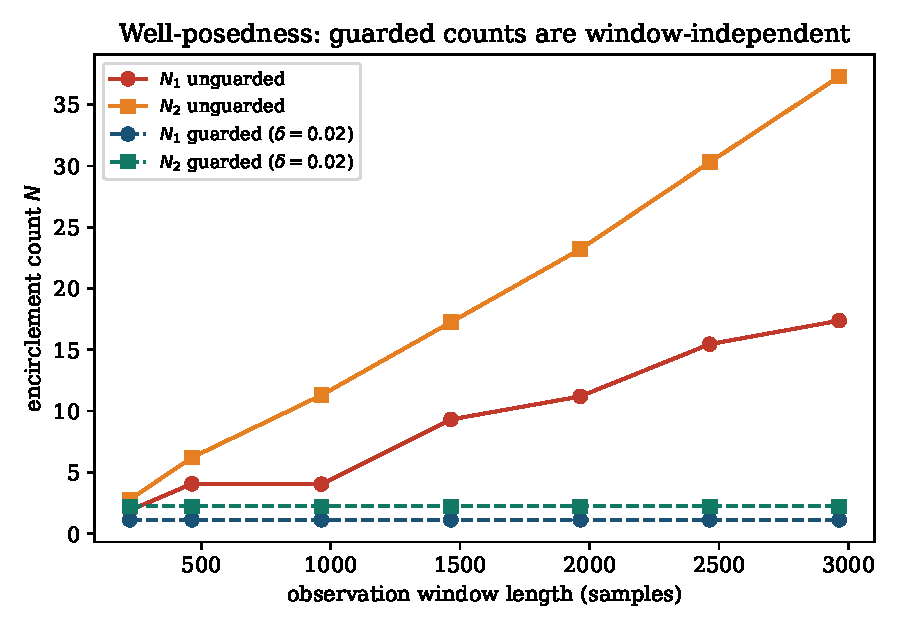
\includegraphics[width=0.95\linewidth]{fig3_wellposed.pdf}
\caption{Window dependence of $N_1, N_2$ on the counterexample plant,
guarded (Definition~\ref{def:guard}) versus unguarded (Definition~1
applied to the raw window). Guarded counts are exactly flat.}
\label{fig:wellposed}
\end{figure}

The remedy is to anchor the window to the settling of the parent signal.

\begin{definition}[Settling-anchored window]\label{def:guard}
Fix $\delta \in (0,1)$ (default $\delta = 0.02$). Let
$k_\delta = 1 + \max\{k : |e_k| > \delta \max_j |e_j|\}$ and truncate all
three trajectories \eqref{eq:plots} at $k_\delta$ before applying
Definition~\ref{def:count}.
\end{definition}

\begin{proposition}[Well-posedness]\label{prop:wellposed}
Under Definition~\ref{def:guard}, the features $\mathbf N$ are independent
of the window length for every window containing the $\delta$-settling
time of $e$, and Proposition~\ref{prop:invariance} continues to hold
($\delta$ is dimensionless and defined on the normalized error).
\end{proposition}

\begin{proof}
All samples beyond $k_\delta$ are discarded, and $k_\delta$ itself depends
only on $e$ up to its $\delta$-settling time; enlarging the window changes
neither. Invariance is preserved because $k_\delta$ is defined through the
ratio $|e_k| / \max_j |e_j|$.
\end{proof}

On the counterexample above, the guarded counts evaluate to
$\mathbf N = (0.12,\, 1.14,\, 2.24)$ on all three windows---identical to
three digits---and, as Section~\ref{sec:battery} shows, the closed-loop
tuning iteration on the same plant converges cleanly once the guard is in
place. The guard is henceforth part of the feature definition; the method
thus carries exactly three dimensionless constants
$(\bar{\mathbf N}, \varepsilon, \delta)$, none of which was adjusted for
any plant in this paper.

\begin{remark}
Proposition~\ref{prop:wellposed} formalizes, and enforces, the practical
requirement that each tuning experiment be observed until the loop
settles. The failure mode it excludes---unbounded winding of a
noise-dominated differenced portrait---is silent and window-dependent,
which is precisely why it deserves a formal guard rather than an
operator's discretion.
\end{remark}

\begin{remark}[Scope of the guard]\label{rem:noise}
\rev{Proposition~\ref{prop:wellposed} assumes a noise-free $e$. With
noise level $\sigma_n$, $k_\delta$ is well defined only if
$\delta \max_j |e_j| \gg \sigma_n$; otherwise $k_\delta$ tracks the last
noise excursion and the divergence can reappear despite the guard---so
$\delta = 0.02$ presumes noise below roughly two percent of the step, a
condition to be checked, not assumed. Likewise, retain enough samples
per transient (tens to a few hundred) that $\Delta e, \Delta^2 e$ are
not quantization-dominated, \revc{and difference the record only from the step instant
onward, so that the reference jump injects no kick into}
$\Gamma_2$.}
\end{remark}

\emph{A stability screen.} The guard, and the counts themselves, presuppose
that the record settles at all: the portraits of a diverging error never
enter the truncation disc, and their winding is an artefact of wherever
the recording happened to stop. Whether the record settles is itself
decidable from the record, with no model and no thresholds.

\begin{definition}[Stability screen]\label{def:screen}
Model the recorded error as emitted by two zero-mean Gaussian generators
switched once at an unknown sample $\tau$. The maximum-likelihood switch
point is
\begin{equation}
\tau^\ast = \arg\max_{\tau}\;
\bigl[-\tau \ln s_1^2(\tau) - (K-\tau)\ln s_2^2(\tau)\bigr],
\end{equation}
where $s_1^2(\tau)$ and $s_2^2(\tau)$ are the mean squares of
$e_0,\dots,e_{\tau-1}$ and $e_\tau,\dots,e_K$ respectively (with $\tau$
ranging over splits that leave at least $10\%$ of the record on each
side). The record is declared \emph{unstable} when
$s_2^2(\tau^\ast) \ge s_1^2(\tau^\ast)$\rev{---the mean-square amplitude
of the segment attributed to the second generator is at least that of
the first---}and \emph{stable} otherwise.
\end{definition}

\rev{A settling response front-loads its energy; a diverging one
back-loads it. \revc{The verdict is invariant to amplitude and time scaling.} Zero-mean moments, rather than
variances about segment means, handle dead time correctly: the delay
plateau is quiet about its own mean but loud about zero, hence read as
part of the transient rather than as a silent first generator; the zero
reference itself is licensed by Assumption~\ref{ass:pid}, since
$K_i > 0$ forces every stable record to end quiet about zero
specifically. A bounded sustained oscillation deliberately
\emph{passes} the screen: a limit cycle has a frequency, is
attributable, and belongs to the band rules, while the screen is
reserved for divergence, which no count can describe.}

%=====================================================================
\section{The tuning rule}
\label{sec:rule}
%=====================================================================

\revc{Order the gains by the frequency band each channel
dominates and write}
\begin{equation}
K^{(0)} = K_i, \qquad K^{(1)} = K_p, \qquad K^{(2)} = K_d,
\label{eq:bandorder}
\end{equation}
so that the band index aligns with the portraits: $N_k$ is the feature
that indicts $K^{(k)}$. Parametrize the gains as multipliers
$F^{(k)} \in [F_{\min}, F_{\max}]$ (defaults $[0.01, 10]$) on any
conservative stabilizing initialization, fix a step $\beta$ (default
$0.1$), and let $\gamma = 1/(1-\beta)$. Each iteration performs one step
test, evaluates $\mathbf N$, and updates the gains.

The rule, in words: \emph{if the record grows rather than decays, halve
all three gains; otherwise scan the portraits from slow to fast; the
first one that loops too much names the gain to turn down one notch, and
every gain below it turns up one notch; if none loops, turn all three
up.} \revc{Table~\ref{tab:rule} is the entire decision logic; the
commissioning craft is recognizable row by row, and the
lower-triangular stencil that names the rule is visible in the arrow
pattern.}

\begin{table}[h]
\centering
\caption{The tuning rule at a glance. The first matching row applies,
top to bottom, once per step test; ``unstable'' is the verdict of
Definition~\ref{def:screen}, ``loops'' means $N_k > \bar N_k$.
$\uparrow$: multiply by $\gamma$;\ $\downarrow$: divide by $\gamma$;\
$\Downarrow$: divide by $2$;\
$\cdot$\,: unchanged. Projections onto $[F_{\min},F_{\max}]$ implied.}
\label{tab:rule}
\setlength{\tabcolsep}{5pt}
\begin{tabular}{lcccl}
\toprule
Condition & $F_i$ & $F_p$ & $F_d$ & craft reading \\
\midrule
unstable & $\Downarrow$ & $\Downarrow$ & $\Downarrow$ &
runaway: halve all \\
$\Gamma_0$ loops & $\downarrow$ & $\cdot$ & $\cdot$ &
slow cycling: less reset \\
$\Gamma_1$ loops & $\uparrow$ & $\downarrow$ & $\cdot$ &
ringing: less gain \\
$\Gamma_2$ loops & $\uparrow$ & $\uparrow$ & $\downarrow$ &
buzzing: less rate \\
none & $\uparrow$ & $\uparrow$ & $\uparrow$ &
all quiet: tighten \\
\bottomrule
\end{tabular}
\end{table}

\begin{center}
\fbox{\begin{minipage}{0.96\linewidth}
\textbf{Procedure.}
\begin{enumerate}[leftmargin=1.4em, itemsep=1pt, topsep=2pt]
\item Close the loop with any gains; conservative ones save iterations.
\item Step the setpoint; record the error $e$.
\item If the record grows rather than decays
(Definition~\ref{def:screen}), halve all gains and go to step~2.
\item Truncate the record where $|e|$ last leaves $2\%$ of its peak
(Definition~\ref{def:guard}).
\item Form the three portraits (Figs.~\ref{fig:init_portraits},
\ref{fig:tuned_portraits}) and count
loops.
\item Apply the matching row of Table~\ref{tab:rule}.
\item Repeat.
\end{enumerate}
\end{minipage}}
\end{center}

\begin{table}[h]
\centering
\caption{Constants and defaults, used unchanged on every plant in this
paper.}
\label{tab:defaults}
\begin{tabular}{lll}
\toprule
Symbol & Meaning & Default \\
\midrule
$\bar{\mathbf N}$ & loop limits & $(0.5, 0.75, 1.0)$ \\
$\varepsilon$ & truncation radius & $0.1$ \\
$\delta$ & settling band & $0.02$ \\
$\beta$ & step size & $0.1$ \\
box & multiplier range & $[0.01, 10]$ \\
\bottomrule
\end{tabular}
\end{table}

Formally, the screen verdict takes precedence: an unstable record
(Definition~\ref{def:screen}) halves all three multipliers and no counts
are evaluated---the portraits of a diverging error carry no usable
information. The backoff is deliberately coarse, $1/2$ rather than
$1/\gamma$: instability is a state to be exited quickly, not corrected
delicately, and fine adjustment is the business of the count rows once a
settling record exists. For a stable record, with the \emph{violated set} and its lowest member
\begin{equation}
V = \{k : N_k > \bar N_k\}, \qquad k_{\min} = \min V
\end{equation}
($k_{\min} = 3$ by convention if $V = \emptyset$), the update reads
\begin{equation}
F^{(k)} \;\leftarrow\;
\begin{cases}
\gamma\, F^{(k)}, & k < k_{\min} \ \text{(raise band)},\\[1mm]
F^{(k)}/\gamma, & k = k_{\min} \ \text{(cut band)},\\[1mm]
F^{(k)}, & k > k_{\min} \ \text{(untouched)},
\end{cases}
\label{eq:triangular}
\end{equation}
for $k_{\min} = 3$ degenerating to raising all bands. \rev{Even when
$|V| > 1$, only $k_{\min}$ is acted on: by the leakage asymmetry of
Section~\ref{sec:feature} it is the only member of $V$ whose guilt is
unambiguous, and bands above it are left alone for lack of evidence, not
out of caution.}

\rev{In loop-shaping terms, the gain profile is pushed up from the
low-frequency end, halting and stepping down at the first band that
objects: a lexicographic bandwidth maximizer, and a fixed-point search
for the boundary of the well-damped set
$\mathcal F = \{\theta : \mathbf N(\theta) \le \bar{\mathbf N}\}$.}

\revc{Three facts follow from \eqref{eq:triangular}. Every band
the rule pours gain into ($k < k_{\min}$) was verified clean in the
current experiment. In logarithmic gain coordinates the corrective
moves form a lower-triangular, unimodular matrix, so their compositions
reach every point of the multiplicative $\gamma$-lattice; an unwanted
compensation is cancelled by a lower-band correction one iteration
later. And the iteration is an implicit attribution test: violations
that clear with the cut at $k_{\min}$ were leakage, violations that
persist are genuine and become the new $k_{\min}$; cutting all of $V$
at once would forgo this inference (Section~\ref{sec:battery}).}

\begin{remark}\label{rem:multichannel}
\rev{Nothing in \eqref{eq:triangular} is specific to three channels:
any controller whose channels dominate disjoint, ascending frequency
bands admits the same construction, with $m$ portraits obtained by
walking the derivative chain and the same triangular stencil. It runs
downward as readily as up---the nested family
$\mathrm{I} \subset \mathrm{PI} \subset \mathrm{PID}$ of
Assumption~\ref{ass:pid} is the scheme at $m = 1, 2, 3$, so restricting
the family restricts the table, not the argument---and fewer bands mean
fewer constraints and a lower-dimensional lattice: on P2, from analogous
conservative starts, the terminal cycle is entered after $41$
experiments for PID, $18$ for PI, and $6$ for a pure I controller.}
\end{remark}

\begin{proposition}[Monotone steering]\label{prop:mono}
\revb{Under Assumption~\ref{ass:plant}, near the boundary of
Proposition~\ref{prop:pair}: (i)~along the uniform direction
$L\mapsto mL$ every count is strictly increasing in $m$; (ii)~each
count $N_k$ is strictly increasing in its own band gain
$K^{(k)}$ at a crossover its band owns; \revc{the cut of the
corrective row of \eqref{eq:triangular} strictly decreases
$N_{k_{\min}}$, and the compensating raises do not cancel it.}}
\end{proposition}

\begin{proof}
\revd{Write $\partial N/\partial\log m =
(\partial N/\partial\zeta)\,(\partial\zeta/\partial\log m)$. The first
factor is negative (Proposition~\ref{prop:law}). For the second: the
phase-crossover frequencies of $mL$ do not move with $m$
($\arg mL = \arg L$), while the gain at each grows linearly in $m$;
the margin to the first touch of $-1$ therefore shrinks strictly, and
near the boundary the critical pair's damping follows it
(Proposition~\ref{prop:pair}). The product
is positive. For~(ii), the same computation runs along the band's own
gain at the crossover its mode owns (Proposition~\ref{prop:band}); the
compensating raises act on lower bands, subdominant in $|C(j\omega)|$
at that crossover, so one rule step keeps the sign of the cut.}
\end{proof}

\begin{remark}[Scope]\label{rem:scope}
\revd{Proposition~\ref{prop:mono} is proved near the stability
boundary and verified over the decision region by measurement. It is
a scalar statement---one count, one loop gain, one crossover---made
possible by the single-frequency mechanism of
Proposition~\ref{prop:pair}. It does not claim that every pole damping
is monotone in every band gain; that matrix-valued statement is false
in general (derivative action adds phase lead as well as
high-frequency gain) and is never used. Nor is the decrease claimed
global in $m$: strong derivative action can raise the dominant damping
over a mid-range of gain---the pair is captured by the controller
zeros, which is what derivative action is for---before the fast
branches take over; the proof needs only the boundary neighbourhood.
On a $14$-plant FOPTD ensemble
with $\tau = L/(L{+}T)\in[0.09,0.90]$, the raise-all direction showed
no above-threshold violations for $\tau\le 0.7$; for delay-dominant
plants ($\tau\gtrsim 0.8$) the dead-time pole comb crowds the critical
pair and isolated count jumps appear, at the $\tau$ where derivative
action is classically marginal \cite{AstromHagglund2004}. There the
iteration stays bounded and parks or cycles.}
\end{remark}

\begin{proposition}[Behaviour of the iteration]\label{prop:conv}
Unconditionally, the iteration is deterministic and its iterates remain in
the multiplier box. \revb{Under Assumption~\ref{ass:plant}, via
Proposition~\ref{prop:mono},} from any
$\theta^0 \in \mathcal F$ the iteration reaches every neighbourhood of
$\partial\mathcal F$ in finitely many steps---or saturates at the box, if
$\mathcal F$ contains it---and thereafter remains within a band of
$\partial\mathcal F$ of width one multiplicative step per gain, on which
it executes a limit cycle.
\end{proposition}

\begin{proof}
Boundedness is by construction of the projections. On $\mathcal F$,
the rule ($V = \emptyset$) multiplies all gains by $\gamma > 1$, an expanding map that
leaves any compact subset of the interior in finitely many steps or
saturates at $F_{\max}$. Once $V \ne \emptyset$, the corrective form of
the rule reduces the lowest violated feature by a fixed factor per step
\revb{(Proposition~\ref{prop:mono})}; when it clears, either the leaked
violations above it clear with it or a genuine one becomes the new
$k_{\min}$ and is reduced in turn, restoring feasibility in finitely
many steps; alternation of expansion and correction confines the
trajectory to the stated band.
\end{proof}

\begin{remark}[Bootstrap from arbitrary gains]\label{rem:bootstrap}
\rev{With the screen row, a stabilizing initialization is a
convenience, not a precondition: plants of Assumption~\ref{ass:plant}
are open-loop stable, so consecutive halvings reach a stabilizing region
within a handful of experiments (or hit $F_{\min}$, a detectable
outcome), after which Proposition~\ref{prop:conv} applies unchanged.
Each backoff costs one experiment on an unstable loop; the mid-test
abort remains the hard safety layer, and a conservative start remains
good practice.}
\end{remark}

\emph{Termination.} \rev{No stopping rule is needed: the expanding form
$V = \emptyset$ is active exactly on $\mathcal F$, so the iteration
never rests and, by Proposition~\ref{prop:conv}, ends in a limit cycle
straddling $\partial\mathcal F$ with excursion one step per gain. The \revc{limits are set so that the regulators visited by the
cycle remain serviceable;}
the iteration may be left running or capped, keeping whichever iterate
it is stopped at. Section~\ref{sec:battery} quotes the last feasible
iterate of each run as a representative of the cycle.} \revb{The monotonicity that drives the proof is no longer
assumed: Proposition~\ref{prop:mono} derives it from the plant class
near the boundary, and Remark~\ref{rem:scope} delimits its reach.
Where the mechanism fails---strong non-minimum-phase behaviour,
resonance, or strongly delay-dominant dynamics---the iteration parks at
a gain bound: detectable, safe, unproductive. It held on every plant
tested. Gains move $\beta = 10\%$ per iteration, and a step test
aborts with rollback if $|e|$ exceeds a configured multiple of the
step.}

\begin{remark}[Bumpless implementation]\label{rem:velocity}
\rev{Because gains change while the loop stays closed, the controller
should be realized in \emph{velocity} (incremental) form,}
\begin{align}
\Delta u_k &= K_p(e_k - e_{k-1}) + K_i T_s e_k
+ \tfrac{K_d}{T_s}(e_k - 2e_{k-1} + e_{k-2}), \notag\\
u_k &= u_{k-1} + \Delta u_k,
\end{align}
\rev{rather than positionally: the increment rides on whatever control
value is currently applied, so a gain change at an iteration
boundary---or a manual-to-automatic transfer---produces no discontinuity
in $u$, and there is no integrator state to reinitialize. This form is
assumed throughout Section~\ref{sec:battery}.}
\end{remark}

%=====================================================================
\section{Validation on a plant battery}
\label{sec:battery}
%=====================================================================

The method---guarded features and the rule of
Table~\ref{tab:rule}---was run on four process-typical plants spanning lag-dominant to
delay-dominant and high-order dynamics:
\begin{align*}
\text{P1 (lag-dominant):} &\quad \tfrac{e^{-s}}{(10s+1)(s+1)^3}, \\
\text{P2 (balanced):} &\quad \tfrac{1.25\,e^{-8s}}{(5s+1)^4}, \\
\text{P3 (delay-dominant):} &\quad \tfrac{e^{-10s}}{(2s+1)(s+1)^3}, \\
\text{P4 (high-order slow):} &\quad \tfrac{e^{-4s}}{(8s+1)^6}.
\end{align*}
All four satisfy
Assumption~\ref{ass:plant}: their open-loop step responses are monotone
with dead time, even where their order exceeds one (Table~\ref{tab:battery}). The runs use the
identical constants
$\bar{\mathbf N} = (0.5, 0.75, 1.0)$, $\varepsilon = 0.1$,
$\delta = 0.02$, $\beta = 0.1$, box $[0.01, 10]$, throughout. In each
case the simulated plant serves exclusively as a stand-in for the physical
process: it generates step responses; the tuner sees only the recorded
error, exactly as on hardware. Initial gains were a nominal design with
proportional and integral gains halved and derivative gain tripled---a
deliberately mis-tuned start exercising the rule at every band position.

\begin{table*}[t]
\centering\small
\caption{Plant battery: initial and returned features, returned
multipliers, iteration at which the returned (last feasible) tuning
occurred, out of $120$. Identical constants throughout; rule
\eqref{eq:triangular}.}
\label{tab:battery}
\begin{tabular}{lllll}
\toprule
Plant & $\mathbf N$ initial & $\mathbf N$ returned & $(F_p, F_i, F_d)$ & iter \\
\midrule
P1 &
$(0.12, 0.13, 0.26)$ & $(0.20, 0.11, 0.78)$ & $(8.10, 10.00, 4.37)^{\ast}$ & 117 \\
P2 &
$(0.12, -0.09, 2.69)$ & $(0.11, 0.23, 0.00)$ & $(1.69, 2.32, 0.25)$ & 114 \\
P3 &
$(0.12, 0.09, 0.00)$ & $(0.46, 0.68, 0.77)$ & $(1.69, 2.87, 0.59)$ & 112 \\
P4 &
$(0.12, 0.11, 0.25)$ & $(0.12, 0.23, 0.00)$ & $(1.37, 2.09, 0.39)$ & 119 \\
\bottomrule
\end{tabular}

\smallskip
\raggedright\footnotesize
$^\ast$Integral multiplier at the box bound: the low band never objects
for this fast, lag-dominant loop, so $F_i$ saturates at $10$, while the
high band supplies the binding constraint ($N_2 = 0.78$)---the partial
saturation case of Proposition~\ref{prop:conv}.
\end{table*}

\rev{Three observations. First, where the mis-tuned derivative channel
creates a fast parasitic mode (P2, P4) the diagnosis is invisible in the
raw response but explicit in $\Gamma_2$ ($N_2 = 2.7$ for P2, lower bands
clean, so the indictment is unambiguous); repeated cuts of band~2 trade
D for P and I until the portrait clears, with feasibility first reached
at iteration $34$. Second, every run ends in the limit cycle of
Proposition~\ref{prop:conv}, feasibility revisited within a few
iterations of the cap---including P4, which churned indefinitely
\emph{without} the guard of Section~\ref{sec:wellposed} and converged
with it. Third, P1 shows partial saturation: its low band never objects,
so $F_i$ rides the box bound while the high band supplies a genuine
constraint.}

\rev{The leakage asymmetry shows live. At iteration $16$ of the P2 run,
$\mathbf N = (0.11,\, 2.08,\, 2.22)$: bands $1$ and $2$ violated with
near-equal counts. One cut of band~$1$ gives $(0.11,\, 0.19,\, 1.25)$:
the mid violation gone, almost half the high count with it (leakage),
and a genuine remainder of $1.25$ persisting as the next $k_{\min}$. A
variant cutting every violated band at once acts on exactly this
unattributable evidence: it drives P2's derivative multiplier to $0.04$
and degrades the returned tuning (IAE $10.7$ against $6.8$ for rule
\eqref{eq:triangular}), similarly on P3, and is therefore not adopted
despite reaching feasibility faster from severely mis-tuned starts.}

\rev{The screen row extends the battery beyond stabilizing starts:
from eight times the nominal design gains on P2---violently
unstable---two halvings settle the response by iteration $2$,
feasibility follows at $56$, and the run returns gains equivalent to
$(0.86,\, 1.06,\, 0.86)$ times the design
(Remark~\ref{rem:bootstrap}).}

\begin{figure*}[t]
\centering
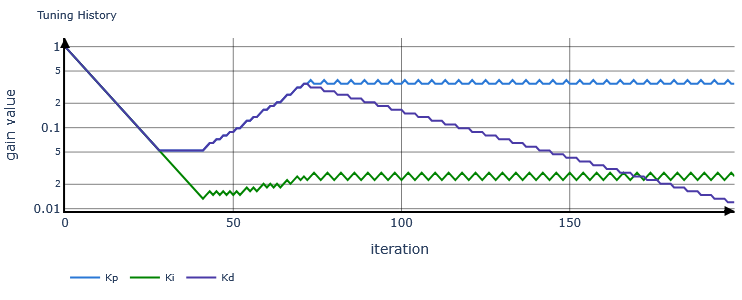
\includegraphics[width=0.85\textwidth]{tuning.png}
\caption{P2, single-band rule: gain trajectories $(K_p, K_i, K_d)$
against iteration, log scale, captured from the running implementation.
After an initial corrective phase the gains settle into the boundary
limit cycle of Proposition~\ref{prop:conv}.}
\label{fig:limitcycle}
\end{figure*}

%=====================================================================
\section{Limits}
%=====================================================================

\rev{\revb{That a band's oscillation is curable by cutting its
gain is derived near the boundary (Proposition~\ref{prop:mono},
Remark~\ref{rem:scope}) rather than presumed;} strong non-minimum-phase or
resonant dynamics break this, visibly and safely, by parking the
iteration at a bound. \revc{The sign of $N_k$ is unused; small negative counts (P2 in
Table~\ref{tab:battery}) are endpoint artefacts of well-damped
records, while a persistent large negative count would signal inverse
response and bear on Assumption~\ref{ass:plant}---left to future
work.} Noise enters the differenced coordinates directly: the
guard excludes settled noise under the condition of
Remark~\ref{rem:noise}, not broadband noise within the transient, and
noisy deployments need filtering outside this paper's scope. Each
iteration needs one settled, undisturbed window; a disturbance corrupts
one test, not the procedure. Single-band action is the price of
attribution: a stable start violating all bands converges through a
sequence of single corrections---from $(2K_p, 3K_i, 4K_d)$ on P4, $74$
iterations to first feasibility---while the attribution-free uniform
backoff is reserved, via the screen, for divergence. Leakage can
misdirect a correction when the true offender sits just below its own
threshold; the stencil self-corrects within a few iterations, at their
cost. The destination is a fast well-damped tuning, not an optimum;
where a criterion matters, it is a sound starting point for
criterion-based refinement.}

%=====================================================================
\section{Conclusion}
%=====================================================================

\revc{Three portraits make under-damping visible band by band; a
winding count makes it a number; a settling-anchored guard makes the
number window-independent; one triangular rule, cutting only the band
whose blame is unambiguous, makes it a decision. The features carry no
units and no clock, so fixed dimensionless constants serve every plant
tested. The iteration is deterministic and bounded unconditionally and
converges to the boundary of the well-damped set under a monotonicity
derived from the plant class.} \revd{The method asks one routine
setpoint step per iteration, needs no model, and shows its work: an
operator watching the three portraits sees every decision the
algorithm makes.}

\section*{Data availability}
Reference implementation, simulation code, and scripts reproducing every
result: \url{https://github.com/ottapav/roboPID-simulator}. An
interactive demonstration is running at
\url{https://robopid-simulator.onrender.com/}.

\bibliographystyle{elsarticle-num}
\begin{thebibliography}{00}
\bibitem{ZN1942} J.G.~Ziegler, N.B.~Nichols, Optimum settings for
automatic controllers, Trans. ASME 64 (1942) 759--768.
\bibitem{AstromHagglund2001} K.J.~\r{A}str\"om, T.~H\"agglund, The future
of PID control, Control Eng. Pract. 9 (11) (2001) 1163--1175.
\bibitem{CohenCoon1953} G.H.~Cohen, G.A.~Coon, Theoretical consideration
of retarded control, Trans. ASME 75 (1953) 827--834.
\bibitem{RiveraIMC} D.E.~Rivera, M.~Morari, S.~Skogestad, Internal model
control: PID controller design, Ind. Eng. Chem. Process Des. Dev. 25 (1)
(1986) 252--265.
\bibitem{AstromHagglund1984} K.J.~\r{A}str\"om, T.~H\"agglund, Automatic
tuning of simple regulators with specifications on phase and amplitude
margins, Automatica 20 (5) (1984) 645--651.
\bibitem{Skogestad2003} S.~Skogestad, Simple analytic rules for model
reduction and PID controller tuning, J. Process Control 13 (4) (2003)
291--309.
\bibitem{AstromHagglund2004} \rev{K.J.~\r{A}str\"om, T.~H\"agglund,
Revisiting the Ziegler--Nichols step response method for PID control,
J. Process Control 14 (6) (2004) 635--650.}
\bibitem{SchlegelCech2005} \rev{M.~Schlegel, M.~\v{C}ech, Computing value
sets from one point of frequency response with applications, in: Proc.
16th IFAC World Congress, Prague, 2005, pp. 325--330.}
\bibitem{Schlegel2011} \rev{M.~Schlegel, Exact revision of the
Ziegler--Nichols frequency response method, in: Proc. IASTED Int. Conf.
Control and Applications, Canc\'un, Mexico, 2011, pp. 121--126.}
\bibitem{HjalmarssonIFT} H.~Hjalmarsson, M.~Gevers, S.~Gunnarsson,
O.~Lequin, Iterative feedback tuning: theory and applications, IEEE
Control Syst. Mag. 18 (4) (1998) 26--41.
\bibitem{CampiVRFT} M.C.~Campi, A.~Lecchini, S.M.~Savaresi, Virtual
reference feedback tuning, Automatica 38 (8) (2002) 1337--1346.
\bibitem{KillingsworthKrstic} N.J.~Killingsworth, M.~Krstic, PID tuning
using extremum seeking, IEEE Control Syst. Mag. 26 (1) (2006) 70--79.
\end{thebibliography}

\end{document}
